% !TEX root = ../../prj4projektrapport.tex
% SKAL STÅ I TOPPEN AF ALLE FILER FOR AT MASTER-filen KOMPILERES 

\section{Kommunikationsmodul}
\label{Kommunikationsmodul}

I starten af projektet var det tænkt at et separat kommunikationsmodul ikke var nødvendigt, da PSoC'en med et tilhørende Ethernetmodul ENC28J60 ville kunne oprette forbindelse til Kontrolmodulet. Der var dog et problem med antallet af Måleenheder på denne måde, da PLC'en kun har ét frit RJ-45 stik ville det stadig være nødvendigt at benytte en switch eller at samle måledata på en enhed og derfra sende dem til PLC'en. Grundet det ikke var muligt at få en switch på værkstedet blev det besluttet at benytte en ekstra microcontroller til at samle data på, denne microcontroller er Kommunikationsmodulet.   

Da det ikke er en nødvendighed for projektet at kommunikationen skal være voldsom hurtig mellem Måleenhederne og Kommunikationsmodulet er der her valgt at benytte UART kommunikation. Denne kommunikationsform er valgt da det før har været benyttet på både Arduino og PSoC, dog uafhængigt af hinanden.

Efter mange timers arbejde med at oprette LAN-kommunikation på en PSoC og det stadig ikke var lykkedes, blev det besluttet at der skulle prøves med en Arduino som Kommunikationsmodul i stedet. 

Kommunikationsmodulet består derfor af en Arduino Mega2560 forbundet til et Ethernet Shield R3. Kommunikationsmodulet skal derved modtage data fra Måleenhederne over UART kommunikation og sende det videre til Kontrolmodulet ved brug af TCP kommunikation. 

Arduinoen opsætter Ethernet Shield'et ved brug af en SPI forbindelse, der oprettes af SPI.h biblioteket, der kaldes som det første i koden. Dernæst er Ethernet.h biblioteket kaldt, for at kunne benytte de meget brugbare funktioner i dette bibliotek\cite{Ethernet}. Der ses herunder et eksempel på nogle af de meget nyttige funktioner, der bruges til at opsætte TCP kommunikation, se figur \ref{EthernetKode}. For mere uddybelse af hele koden refereres der til dokumentationen\footnote{Projektdokumentation, 10.3, Kommunikationsmodul}.

\lstset{caption={Ethernet},label={EthernetKode}}
\begin{lstlisting} % Start your code-block

// Skrevet i den globale del af koden:
#include <SPI.h>
#include <Ethernet.h>

byte mac[] = {0x90, 0xA2, 0xDA, 0x0F, 0x1B, 0x82};   // MAC Address
byte ip[] = {192, 168, 0, 129};                // Network Address


EthernetServer server = EthernetServer(27015);


// Skrevet i setup delen af koden:
Ethernet.begin(mac,ip);
server.begin();


\end{lstlisting}


Kommunikationen over TCP mellem Kommunikationsmodul og Kontrolmodulet starter ved at Kontrolmodulet opretter forbindelse til Kommunikationsmodul. Dette detekteres af Kommunikationsmodulet og den starter med at modtage request kommandoer fra Kontrolmodulet. Hver Måleenhed har en forskellig request kommando, i dette tilfælde er der brugt 'req1' og req2' for de to Måleenheder. Når Kommunikationsmodulet modtager 'req1' sendes dataene fra den tilsvarende Måleenhed til Kontrolmodulet. Måledataene sendes videre præcis som de er modtaget, det vil sige at hver måling sendes som to 8-bit integers, men da alle målinger sendes efter hinanden refereres de oftest til som måledata. Se figur \ref{fig:TCPProtokol}.

\begin{figure}[H] % (alternativt [H])
	\centering
	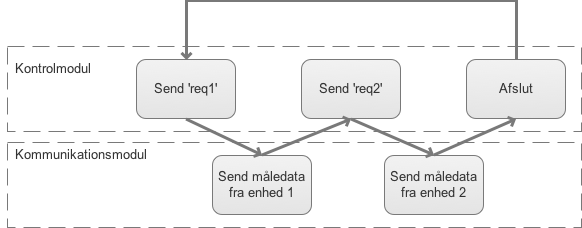
\includegraphics[width=0.7\textwidth]{Figure/TCPProtokol}
	\caption{Protokol for kommunikation mellem kommunikationsmodul og kontrolmodul}
	\label{fig:TCPProtokol}
\end{figure}



